\documentclass[11pt,a4paper]{article}
\usepackage[utf8]{inputenc}
\usepackage[T1]{fontenc}
\usepackage{amsmath,amssymb}
\usepackage{booktabs}
\usepackage{graphicx}
\usepackage{xcolor}
\usepackage{hyperref}
\usepackage{tikz}
\usetikzlibrary{shapes.geometric, arrows.meta, positioning, calc}
\usepackage{algorithm}
\usepackage{algpseudocode}
\usepackage{geometry}
\geometry{margin=1in}

\hypersetup{
    colorlinks=true,
    linkcolor=blue,
    urlcolor=blue,
}

% Define colors
\definecolor{baselinecolor}{RGB}{66, 133, 244}
\definecolor{optimizedcolor}{RGB}{52, 168, 83}
\definecolor{convexcolor}{RGB}{234, 67, 53}
\definecolor{greedycolor}{RGB}{251, 188, 4}

% TikZ styles
\tikzstyle{startstop} = [rectangle, rounded corners, minimum width=3cm, minimum height=1cm, text centered, draw=black, fill=gray!20]
\tikzstyle{process} = [rectangle, minimum width=3cm, minimum height=1cm, text centered, draw=black, fill=blue!10]
\tikzstyle{decision} = [diamond, minimum width=3cm, minimum height=1cm, text centered, draw=black, fill=yellow!20, aspect=2]
\tikzstyle{arrow} = [thick,->,>=stealth]

\title{\textbf{Simulation Workflow \& Optimization Methods}\\[0.5em]\large Energy Trading System Documentation}
\author{}
\date{}

\begin{document}

\maketitle
\tableofcontents
\newpage

%=============================================================================
\section{Simulation Overview}
%=============================================================================

The Energy Trading System simulation runs two parallel scenarios for comparison:

\subsection{Baseline Simulation}
Households operate independently without peer-to-peer (P2P) trading. Each household can only:
\begin{itemize}
    \item Use their own solar production
    \item Store/retrieve energy from their battery
    \item Buy from or sell to the city grid
\end{itemize}

\subsection{Optimized Simulation}
Households participate in P2P energy trading using one of the optimization algorithms. They can:
\begin{itemize}
    \item Trade energy with neighboring households
    \item Optimize battery usage based on forecasts
    \item Minimize costs through strategic trading decisions
\end{itemize}

%=============================================================================
\section{Workflow Stages}
%=============================================================================

\subsection{Stage 1: Initialization}

The simulation begins with the following initialization steps:

\begin{enumerate}
    \item Load household data (production/consumption profiles)
    \item Create battery instances (Simple, Shared, or Central)
    \item Initialize blockchain for P2P transaction logging
    \item Set up forecaster and price estimator
    \item Configure optimizer (Convex or Greedy)
    \item Load grid capacity constraints
\end{enumerate}

\subsection{Stage 2: Step-by-Step Execution}

For each simulation step (typically representing a time period like 30 minutes or 1 hour), both simulations run in parallel:

\begin{figure}[h]
\centering
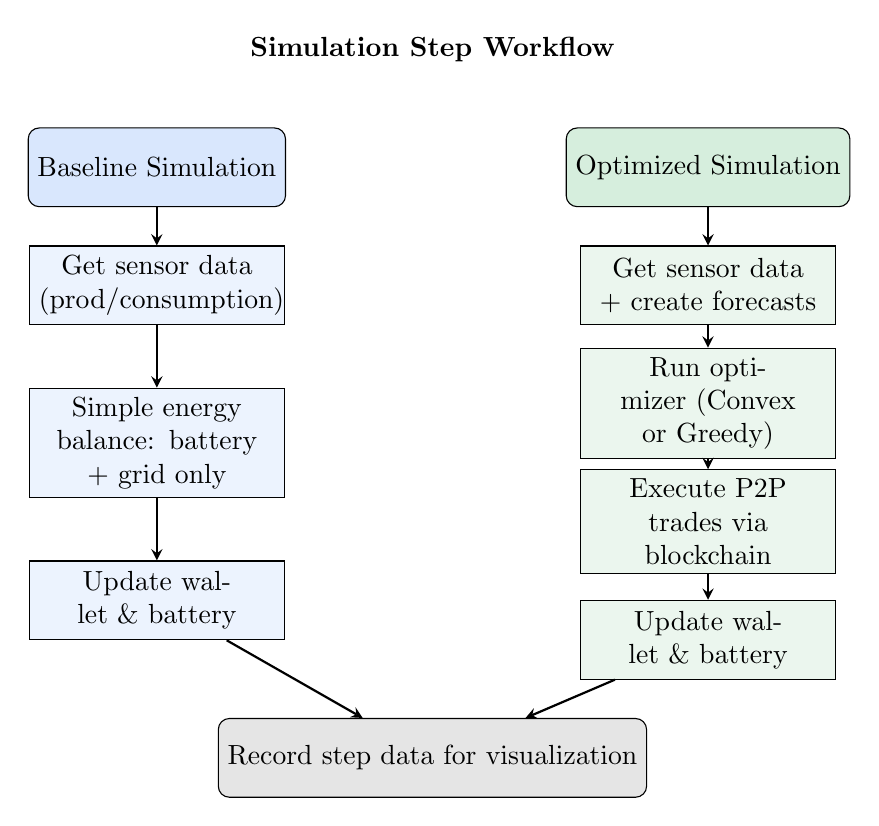
\begin{tikzpicture}[node distance=1.5cm, auto]
    % Title
    \node[font=\bfseries] (title) at (0, 0.5) {Simulation Step Workflow};
    
    % Left side - Baseline
    \node[startstop, fill=baselinecolor!20] (baseline) at (-3.5, -1) {Baseline Simulation};
    \node[process, fill=baselinecolor!10, text width=3cm] (b1) at (-3.5, -2.5) {Get sensor data (prod/consumption)};
    \node[process, fill=baselinecolor!10, text width=3cm] (b2) at (-3.5, -4.5) {Simple energy balance: battery + grid only};
    \node[process, fill=baselinecolor!10, text width=3cm] (b3) at (-3.5, -6.5) {Update wallet \& battery};
    
    % Right side - Optimized
    \node[startstop, fill=optimizedcolor!20] (optimized) at (3.5, -1) {Optimized Simulation};
    \node[process, fill=optimizedcolor!10, text width=3cm] (o1) at (3.5, -2.5) {Get sensor data + create forecasts};
    \node[process, fill=optimizedcolor!10, text width=3cm] (o2) at (3.5, -4) {Run optimizer (Convex or Greedy)};
    \node[process, fill=optimizedcolor!10, text width=3cm] (o3) at (3.5, -5.5) {Execute P2P trades via blockchain};
    \node[process, fill=optimizedcolor!10, text width=3cm] (o4) at (3.5, -7) {Update wallet \& battery};
    
    % Merge
    \node[startstop, fill=gray!20] (merge) at (0, -8.5) {Record step data for visualization};
    
    % Arrows - Baseline
    \draw[arrow] (baseline) -- (b1);
    \draw[arrow] (b1) -- (b2);
    \draw[arrow] (b2) -- (b3);
    \draw[arrow] (b3) -- (merge);
    
    % Arrows - Optimized
    \draw[arrow] (optimized) -- (o1);
    \draw[arrow] (o1) -- (o2);
    \draw[arrow] (o2) -- (o3);
    \draw[arrow] (o3) -- (o4);
    \draw[arrow] (o4) -- (merge);
\end{tikzpicture}
\caption{Parallel execution of baseline and optimized simulations at each step}
\end{figure}

\subsection{Stage 3: Data Collection \& Results}

After all steps complete:
\begin{itemize}
    \item Both simulations' data is collected in \texttt{SimulationDataCollector}
    \item Results are exported to CSV files for analysis
    \item Metrics are computed: savings, P2P volume, equity (Gini coefficient)
\end{itemize}

%=============================================================================
\section{Optimization Methods}
%=============================================================================

\subsection{Convex Optimizer}

The Convex Optimizer uses \textbf{CVXPY} (a Python library for convex optimization) to solve a multi-timestep optimization problem that minimizes total community energy costs.

\subsubsection{Mathematical Formulation}

\paragraph{Decision Variables}
\begin{align}
    G_{\text{buy}}[i,t] &\geq 0 \quad \text{Grid purchases for household } i \text{ at time } t \\
    G_{\text{sell}}[i,t] &\geq 0 \quad \text{Grid sales for household } i \text{ at time } t \\
    B[i,t] &\geq 0 \quad \text{Battery state for household } i \text{ at time } t \\
    B_{\text{charge}}[i,t] &\geq 0 \quad \text{Battery charging amount} \\
    B_{\text{discharge}}[i,t] &\geq 0 \quad \text{Battery discharging amount} \\
    \text{net}_{\text{P2P}}[i,t] &\in \mathbb{R} \quad \text{Net P2P position (+ = seller, - = buyer)}
\end{align}

\paragraph{Constraints}

\textbf{Energy Balance:}
\begin{equation}
    P_i(t) + G_{\text{buy}}[i,t] + B_{\text{discharge}}[i,t] = C_i(t) + G_{\text{sell}}[i,t] + B_{\text{charge}}[i,t] + \text{net}_{\text{P2P}}[i,t]
\end{equation}
where $P_i(t)$ is production and $C_i(t)$ is consumption.

\textbf{P2P Market Balance:}
\begin{equation}
    \sum_{i=1}^{N} \text{net}_{\text{P2P}}[i,t] = 0 \quad \forall t
\end{equation}

\textbf{Grid Capacity:}
\begin{align}
    \sum_{i=1}^{N} G_{\text{buy}}[i,t] &\leq \text{ImportCapacity}(t) \\
    \sum_{i=1}^{N} G_{\text{sell}}[i,t] &\leq \text{ExportCapacity}(t)
\end{align}

\textbf{Battery Dynamics:}
\begin{equation}
    B[i,t+1] = B[i,t] + \eta_c \cdot B_{\text{charge}}[i,t] - \frac{B_{\text{discharge}}[i,t]}{\eta_d}
\end{equation}
where $\eta_c$ and $\eta_d$ are charge and discharge efficiencies.

\paragraph{Objective Function}

\begin{equation}
\begin{aligned}
    \min \quad & \sum_{i,t} G_{\text{buy}}[i,t] \cdot p_{\text{buy}}(t) - \sum_{i,t} G_{\text{sell}}[i,t] \cdot p_{\text{sell}}(t) \\
    & + \lambda_1 \sum_{i,t} |\text{net}_{\text{P2P}}[i,t]| + \lambda_2 \sum_{i,t} [\text{wallet}[i,t]]^- + \lambda_3 \cdot \text{TransactionCost}
\end{aligned}
\end{equation}

\subsubsection{Key Parameters}

\begin{table}[h]
\centering
\begin{tabular}{lll}
\toprule
\textbf{Parameter} & \textbf{Description} & \textbf{Default} \\
\midrule
\texttt{solver} & Optimization solver (CLARABEL, ECOS, OSQP, SCS) & CLARABEL \\
\texttt{warm\_start} & Reuse previous solution to speed up solving & True \\
\texttt{p2p\_transaction\_cost} & Cost per P2P transaction & 0.5 \\
\texttt{min\_trade\_threshold} & Minimum kWh for a trade & 0.1 \\
\texttt{max\_neighbors} & Limit trading to N nearest neighbors & None (all) \\
\bottomrule
\end{tabular}
\caption{Convex optimizer parameters}
\end{table}

\subsubsection{Advantages and Disadvantages}

\textbf{Advantages:}
\begin{itemize}
    \item[\textcolor{green}{\checkmark}] Finds globally optimal or near-optimal solutions
    \item[\textcolor{green}{\checkmark}] Considers future timesteps for better planning
    \item[\textcolor{green}{\checkmark}] Handles complex constraints elegantly
    \item[\textcolor{green}{\checkmark}] Mathematically rigorous
\end{itemize}

\textbf{Disadvantages:}
\begin{itemize}
    \item[\textcolor{red}{$\times$}] Computationally expensive: $O(N^2 T)$ complexity
    \item[\textcolor{red}{$\times$}] Requires specialized solver libraries
    \item[\textcolor{red}{$\times$}] May be slow for large numbers of households
    \item[\textcolor{red}{$\times$}] More complex to understand and debug
\end{itemize}

%-----------------------------------------------------------------------------
\subsection{Greedy Optimizer}

The Greedy Optimizer uses a fast heuristic algorithm that makes locally optimal decisions at each timestep without looking ahead.

\subsubsection{Algorithm}

\begin{algorithm}[H]
\caption{Greedy P2P Energy Trading}
\begin{algorithmic}[1]
\For{each household $i$}
    \State $\text{net}_i \gets P_i - C_i$ \Comment{Production minus consumption}
    \If{$\text{net}_i > 0$ \textbf{and} battery below target}
        \State Charge battery first
        \State $\text{net}_i \gets \text{net}_i - \text{charge\_amount}$
    \ElsIf{$\text{net}_i < 0$ \textbf{and} battery has reserves}
        \State Discharge battery first
        \State $\text{net}_i \gets \text{net}_i + \text{discharge\_amount}$
    \EndIf
\EndFor
\State
\State $\text{Sellers} \gets \{i : \text{net}_i > \text{threshold}\}$
\State $\text{Buyers} \gets \{i : \text{net}_i < -\text{threshold}\}$
\State Sort Sellers by surplus (largest first)
\State Sort Buyers by deficit (largest first)
\State
\For{each buyer $b \in \text{Buyers}$}
    \For{each seller $s \in \text{Sellers}$}
        \If{$s$ is neighbor of $b$}
            \State $\text{trade} \gets \min(\text{demand}_b, \text{supply}_s)$
            \If{$\text{trade} \geq \text{threshold}$}
                \State Execute trade between $b$ and $s$
                \State Update remaining supply and demand
            \EndIf
        \EndIf
    \EndFor
\EndFor
\State
\State Remaining surplus $\rightarrow$ Sell to city grid
\State Remaining deficit $\rightarrow$ Buy from city grid
\end{algorithmic}
\end{algorithm}

\subsubsection{Key Parameters}

\begin{table}[h]
\centering
\begin{tabular}{lll}
\toprule
\textbf{Parameter} & \textbf{Description} & \textbf{Default} \\
\midrule
\texttt{battery\_target\_pct} & Target battery level to maintain (0--1) & 0.5 \\
\texttt{p2p\_price\_factor} & P2P price as fraction of grid buy price & 0.80 \\
\texttt{p2p\_transaction\_cost} & Minimum savings required for P2P trade & 0.25 \\
\texttt{min\_trade\_threshold} & Minimum kWh for a trade & 0.5 \\
\texttt{max\_neighbors} & Limit trading to N nearest neighbors & None (all) \\
\bottomrule
\end{tabular}
\caption{Greedy optimizer parameters}
\end{table}

\subsubsection{Advantages and Disadvantages}

\textbf{Advantages:}
\begin{itemize}
    \item[\textcolor{green}{\checkmark}] Very fast: $O(N \log N)$ per timestep
    \item[\textcolor{green}{\checkmark}] Easy to understand and debug
    \item[\textcolor{green}{\checkmark}] Naturally prevents simultaneous buy/sell
    \item[\textcolor{green}{\checkmark}] Works well for real-time and large-scale simulations
    \item[\textcolor{green}{\checkmark}] No external solver dependencies
\end{itemize}

\textbf{Disadvantages:}
\begin{itemize}
    \item[\textcolor{red}{$\times$}] May not find globally optimal solution
    \item[\textcolor{red}{$\times$}] Doesn't consider future timesteps (myopic)
    \item[\textcolor{red}{$\times$}] Simpler battery strategy
    \item[\textcolor{red}{$\times$}] Order-dependent matching may miss better pairings
\end{itemize}

%=============================================================================
\section{Comparison}
%=============================================================================

\begin{table}[h]
\centering
\begin{tabular}{lcc}
\toprule
\textbf{Aspect} & \textbf{Convex Optimizer} & \textbf{Greedy Optimizer} \\
\midrule
Speed & Slow ($O(N^2 T)$) & Fast ($O(N \log N)$) \\
Optimality & Global/near-optimal & Locally optimal \\
Lookahead & Multi-timestep & Single timestep \\
Complexity & High & Low \\
Dependencies & CVXPY + solver & None \\
Scalability & Limited ($\sim$50 households) & Excellent (1000+ households) \\
Battery Strategy & Sophisticated & Simple (target-based) \\
Debugging & Difficult & Easy \\
\bottomrule
\end{tabular}
\caption{Side-by-side comparison of optimization methods}
\end{table}

%=============================================================================
\section{Choosing an Optimizer}
%=============================================================================

\begin{figure}[h]
\centering
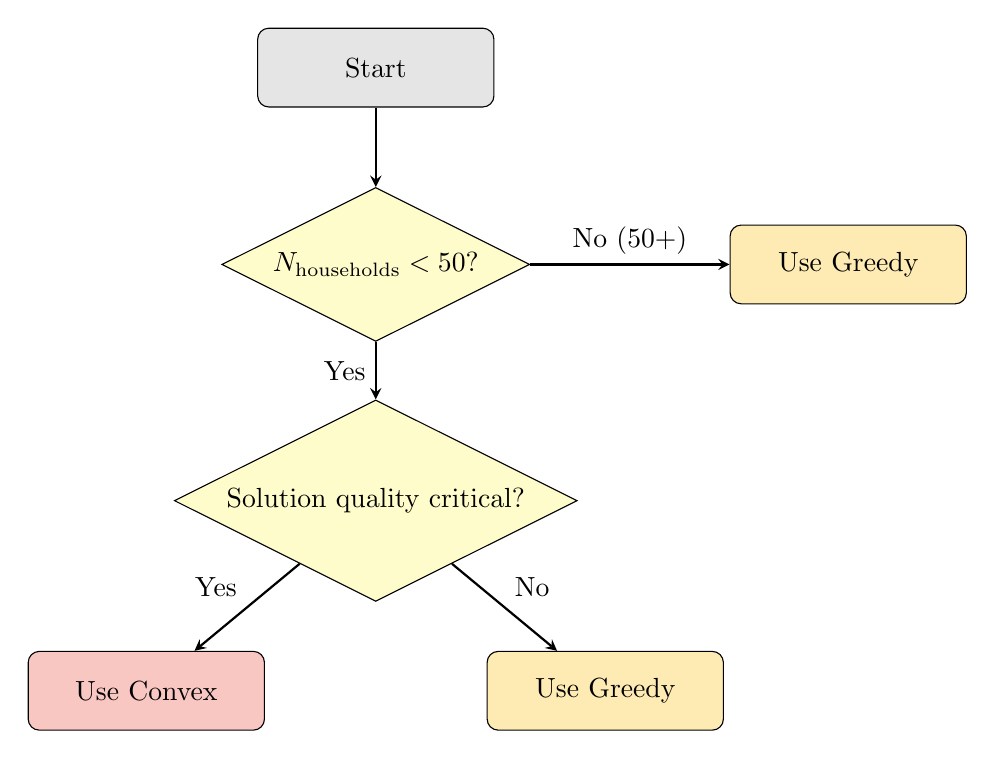
\begin{tikzpicture}[node distance=2cm, auto]
    % Start
    \node[startstop] (start) {Start};
    
    % First decision
    \node[decision, below of=start, yshift=-0.5cm] (d1) {$N_{\text{households}} < 50$?};
    
    % Right branch - many households
    \node[startstop, right of=d1, xshift=4cm, fill=greedycolor!30] (greedy1) {Use Greedy};
    
    % Second decision
    \node[decision, below of=d1, yshift=-1cm] (d2) {Solution quality critical?};
    
    % Final nodes
    \node[startstop, below left of=d2, xshift=-1.5cm, yshift=-1cm, fill=convexcolor!30] (convex) {Use Convex};
    \node[startstop, below right of=d2, xshift=1.5cm, yshift=-1cm, fill=greedycolor!30] (greedy2) {Use Greedy};
    
    % Arrows
    \draw[arrow] (start) -- (d1);
    \draw[arrow] (d1) -- node[above] {No (50+)} (greedy1);
    \draw[arrow] (d1) -- node[left] {Yes} (d2);
    \draw[arrow] (d2) -- node[above left] {Yes} (convex);
    \draw[arrow] (d2) -- node[above right] {No} (greedy2);
\end{tikzpicture}
\caption{Decision flowchart for optimizer selection}
\end{figure}

\subsection{When Each Optimizer Shines}

\textbf{Convex Optimizer} is better when:
\begin{itemize}
    \item You have a small to medium number of households ($< 50$)
    \item Solution quality is more important than speed
    \item You need to respect complex constraints
    \item Planning horizon matters (e.g., time-of-use pricing)
\end{itemize}

\textbf{Greedy Optimizer} is better when:
\begin{itemize}
    \item You have many households (100+)
    \item Real-time decisions are needed
    \item Simplicity and interpretability are valued
    \item Computational resources are limited
\end{itemize}

%=============================================================================
\section{Configuration}
%=============================================================================

In the GUI or parameters file, set the optimizer type:

\begin{verbatim}
{
  "optimizer": {
    "optimizer_type": "convex",  // or "greedy"
    "p2p_transaction_cost": 0.5,
    "min_trade_threshold": 0.1,
    "solver": "CLARABEL",
    "warm_start": true,
    "max_neighbors": null,
    "battery_target_pct": 0.5,
    "p2p_price_factor": 0.8
  }
}
\end{verbatim}

%=============================================================================
\section{Typical Results}
%=============================================================================

Both optimizers should show improvements over the baseline in terms of:

\begin{enumerate}
    \item \textbf{Lower energy costs}: P2P trading reduces grid purchases at higher prices
    \item \textbf{Higher revenue}: Sellers get better prices than grid sell rates
    \item \textbf{More equitable distribution}: P2P spreads benefits across the community
    \item \textbf{Better battery utilization}: Optimized charging/discharging strategies
\end{enumerate}

The Convex optimizer typically achieves 5--15\% better cost savings than Greedy, but at significantly higher computational cost. For most practical applications, the Greedy optimizer provides an excellent balance of performance and efficiency.

\end{document}
